\documentclass{article}\usepackage[]{graphicx}\usepackage[]{color}
%% maxwidth is the original width if it is less than linewidth
%% otherwise use linewidth (to make sure the graphics do not exceed the margin)
\makeatletter
\def\maxwidth{ %
  \ifdim\Gin@nat@width>\linewidth
    \linewidth
  \else
    \Gin@nat@width
  \fi
}
\makeatother

\definecolor{fgcolor}{rgb}{0.345, 0.345, 0.345}
\newcommand{\hlnum}[1]{\textcolor[rgb]{0.686,0.059,0.569}{#1}}%
\newcommand{\hlstr}[1]{\textcolor[rgb]{0.192,0.494,0.8}{#1}}%
\newcommand{\hlcom}[1]{\textcolor[rgb]{0.678,0.584,0.686}{\textit{#1}}}%
\newcommand{\hlopt}[1]{\textcolor[rgb]{0,0,0}{#1}}%
\newcommand{\hlstd}[1]{\textcolor[rgb]{0.345,0.345,0.345}{#1}}%
\newcommand{\hlkwa}[1]{\textcolor[rgb]{0.161,0.373,0.58}{\textbf{#1}}}%
\newcommand{\hlkwb}[1]{\textcolor[rgb]{0.69,0.353,0.396}{#1}}%
\newcommand{\hlkwc}[1]{\textcolor[rgb]{0.333,0.667,0.333}{#1}}%
\newcommand{\hlkwd}[1]{\textcolor[rgb]{0.737,0.353,0.396}{\textbf{#1}}}%

\usepackage{framed}
\makeatletter
\newenvironment{kframe}{%
 \def\at@end@of@kframe{}%
 \ifinner\ifhmode%
  \def\at@end@of@kframe{\end{minipage}}%
  \begin{minipage}{\columnwidth}%
 \fi\fi%
 \def\FrameCommand##1{\hskip\@totalleftmargin \hskip-\fboxsep
 \colorbox{shadecolor}{##1}\hskip-\fboxsep
     % There is no \\@totalrightmargin, so:
     \hskip-\linewidth \hskip-\@totalleftmargin \hskip\columnwidth}%
 \MakeFramed {\advance\hsize-\width
   \@totalleftmargin\z@ \linewidth\hsize
   \@setminipage}}%
 {\par\unskip\endMakeFramed%
 \at@end@of@kframe}
\makeatother

\definecolor{shadecolor}{rgb}{.97, .97, .97}
\definecolor{messagecolor}{rgb}{0, 0, 0}
\definecolor{warningcolor}{rgb}{1, 0, 1}
\definecolor{errorcolor}{rgb}{1, 0, 0}
\newenvironment{knitrout}{}{} % an empty environment to be redefined in TeX

\usepackage{alltt}

\usepackage{multicol}
\usepackage{geometry}
\usepackage{amsmath}

\geometry{
 a4paper,
 total={210mm,297mm},
 left=20mm,
 right=20mm,
 top=20mm,
 bottom=20mm,
 }
\IfFileExists{upquote.sty}{\usepackage{upquote}}{}
\begin{document}

\title{GTEx expression data\\-\\
        Rainet project}
\author{Diogo Ribeiro, Lionel Spinelli, Andreas Zanzoni, Christine Brun}
\maketitle

\section{Introduction} 

We plan to use the GTEx V6 dataset (http://gtexportal.org), Human genome-wide RNA-seq expression data, to add RNA expression information in our RAINET database. 
The purpose is to use the expression to filter out Protein-RNA interactions that unlikely to occur in vivo. We will apply a threshold of expression value to ascertain the potential presence of each protein and RNA in a certain tissue, and excluded interactions where one or both of the interaction partners are missing. 
We will extrapolate the protein presence or absence by the expression of their respective mRNA. It as been shown (Vogel, Christine Marcotte, Edward M. 2012) that prediction of protein presence (but not the protein abundance) is accurate when its mRNA molecules are present at a certain level. \par
The GTEx dataset contains full RNA-seq experiments done on hundreds of individuals, and retrieved from several physical locations / tissues. 
The GTEx project provides downloadable data where the reads have been mapped to human genome and rpkm values were calculated for each GENCODE (v19) transcript (note that this includes all types of RNAs: mRNAs, lncRNAs, snoRNAs, etc).
They provide several files, among them the description of the individual RNA-seq samples, including the tissue and body site:
GTEx\_Data\_V6\_Annotations\_SampleAttributesDS.txt. \par
The file with the rpkm values contains values for each transcript for each sample:
GTEx\_Analysis\_v6\_RNA-seq\_Flux1.6\_transcript\_rpkm.txt. \par
For insertion of expression data into our RAINET database we want to transform the GTEx data to have a single expression value for each RNA-tissue pair, therefore, exclude the sample/individual dimension from the data. 
We will first perform a rough analysis of expression values distributions across samples in order to reach the best solution for processing this data.

\section{Sample numbers per tissue}

Number of samples per tissue using the whole GTEx\_Data\_V6\_Annotations\_SampleAttributesDS.txt
file with the attribute SMTSD (the more-specific tissue terms, e.g. brain breakdown into brain subregions).

\begin{knitrout}
\definecolor{shadecolor}{rgb}{0.969, 0.969, 0.969}\color{fgcolor}
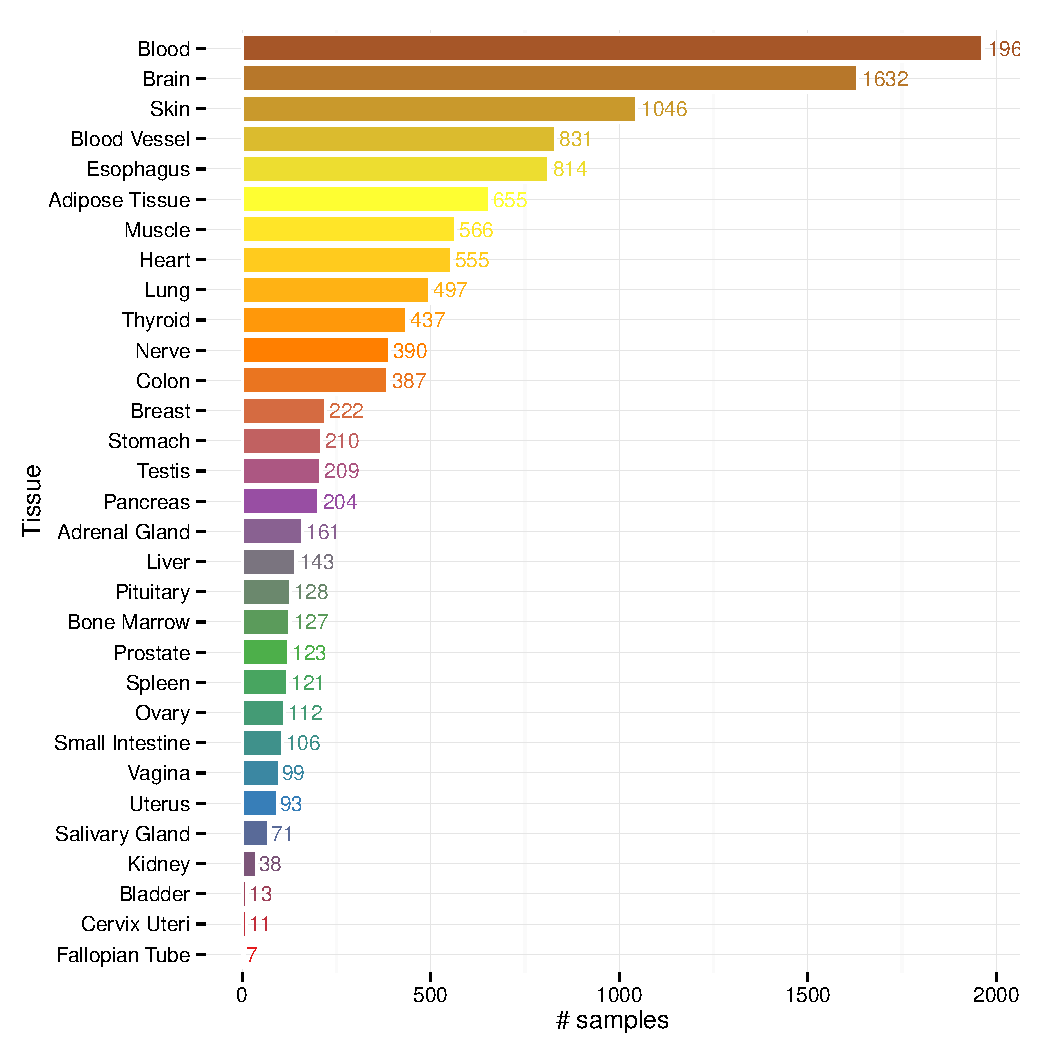
\includegraphics[width=\maxwidth]{figure/samples_per_tissue-1} 
\begin{kframe}\begin{verbatim}
## [1] "Total # of tissues :  49"
## [1] "Total # of samples :  8527"
\end{verbatim}
\end{kframe}
\end{knitrout}

We can see that number of samples per tissue is highly variable. Perhaps this should be considered in the further analysis. Furthermore, some tissues contain only a limited number of samples. \par
We decided to exclude tissues with less than 30 samples (i.e. we excluded the four bottom tissues in the above plot).

\section{Expression variability per tissue}

Following is the distribution of all the expression values per tissue of 50 randomly sampled transcripts (out of 195.747 thousand from GENCODE), sampled from the whole GTEx rpkm file. The boxplot contains the distribution of expression values for the sample transcripts using all available samples (e.g. thousands in brain, a handful in Fallopian tube). \par 

\begin{knitrout}
\definecolor{shadecolor}{rgb}{0.969, 0.969, 0.969}\color{fgcolor}\begin{kframe}
\begin{verbatim}
## [1] "ALL SAMPLES: summary(expression_df$value[expression_df$variable == Muscle − Skeletal]"
##    Min. 1st Qu.  Median    Mean 3rd Qu.    Max. 
##                                                 
## [1] "ALL SAMPLES: summary(expression_df$value[expression_df$variable == Fallopian Tube]"
##    Min. 1st Qu.  Median    Mean 3rd Qu.    Max. 
## 
\end{verbatim}
\end{kframe}
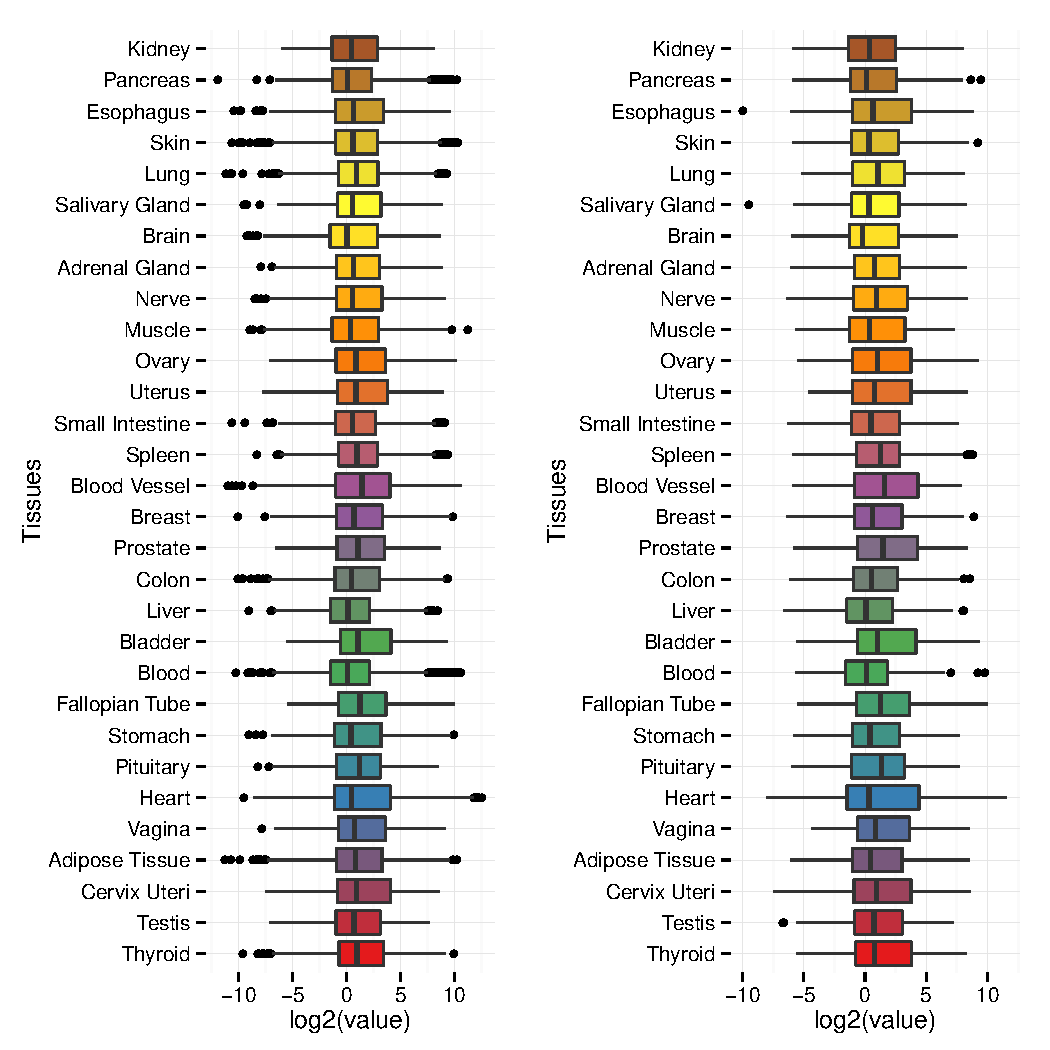
\includegraphics[width=\maxwidth]{figure/expression_per_tissue-1} 

\end{knitrout}

Note that the scale is in log2, and that the rpkm values have a very large spread. However, this spread occurs in all tissues and does not seem to be different in tissues with a larger sample number.\par

\section{Expression distribution per transcript}

We selected 5 tissues with different sample numbers (2 with highest, 1 medium, 2 with lowest sample numbers), randomly selected 12 transcripts and plotted their RPKM value distribution, using all available samples. Note that many transcript have 0 or close to 0 RPKM (Note: there is bug in ggplot density graphics when all RPKMs are zero) in all addressed tissues. 

\begin{knitrout}
\definecolor{shadecolor}{rgb}{0.969, 0.969, 0.969}\color{fgcolor}
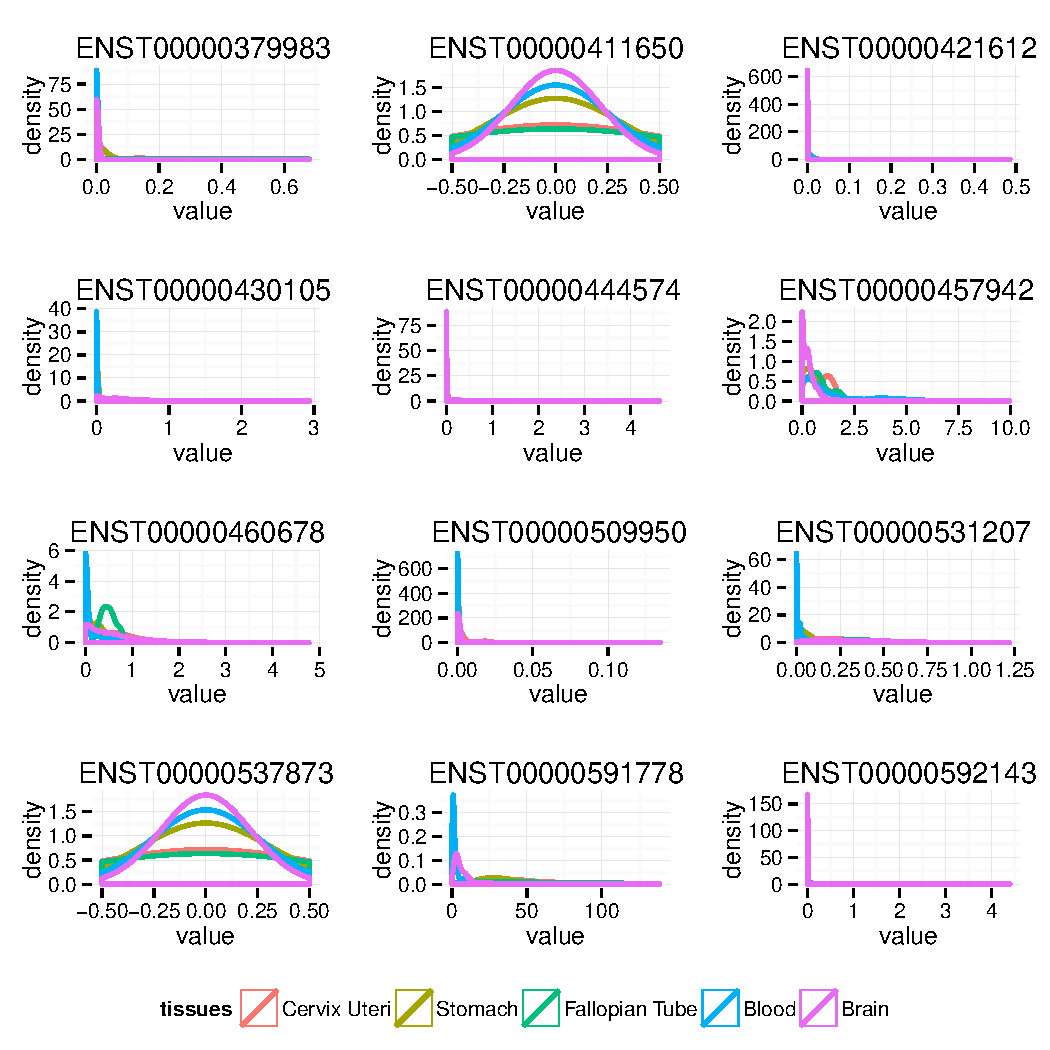
\includegraphics[width=\maxwidth]{figure/density_plot_example_transcripts-1} 

\end{knitrout}

The distributions are highly variable between transcripts and between each tissue, as expected biologically, however they should not be massively variable between samples (i.e. between individuals). 

\section{Average expression of transcripts per tissue}

To merge sample values within the same tissue and transcript, we can calculate their mean. However, some transcripts have highly variable rpkm values, as denoted by the coefficient variation histogram below. If we exclude samples with outlier values (values outside of the range: Q1 - 1.5 * IQR : Q3 + 1.5 * IQR ). The coefficient of variation is largely reduced when applying this filter (see lower histogram). We observed that this filtering removes on average ~4\% of samples for each transcript. Note that the outlier removal is performed for each transcript-tissue, based on their specific rpkm distribution. Note: for better visualisation, these plots do not display values equal to zero, which are the majority. \par
Below are the distributions of mean RPKM values among all transcripts and all tissues, before and after the outlier filtering. As expected the mean is decrease when applying the filtering.\par 
The blue horizontal lines represent either the mean, the red lines represent the noise cutoff of 0.1 RPKM suggested in the GTEx papers.\par
Note: using xlimit at 5 rpkm for better visualisation, due to the large spread of values.\par

\begin{knitrout}
\definecolor{shadecolor}{rgb}{0.969, 0.969, 0.969}\color{fgcolor}\begin{kframe}
\begin{verbatim}
## 
Read 16.8% of 9629480 rows
Read 32.2% of 9629480 rows
Read 47.5% of 9629480 rows
Read 62.6% of 9629480 rows
Read 77.0% of 9629480 rows
Read 90.9% of 9629480 rows
Read 9629480 rows and 7 (of 7) columns from 0.641 GB file in 00:00:08
## 
Read 11.6% of 9629480 rows
Read 28.9% of 9629480 rows
Read 47.0% of 9629480 rows
Read 64.7% of 9629480 rows
Read 82.4% of 9629480 rows
Read 9629480 rows and 7 (of 7) columns from 0.609 GB file in 00:00:07
\end{verbatim}
\end{kframe}
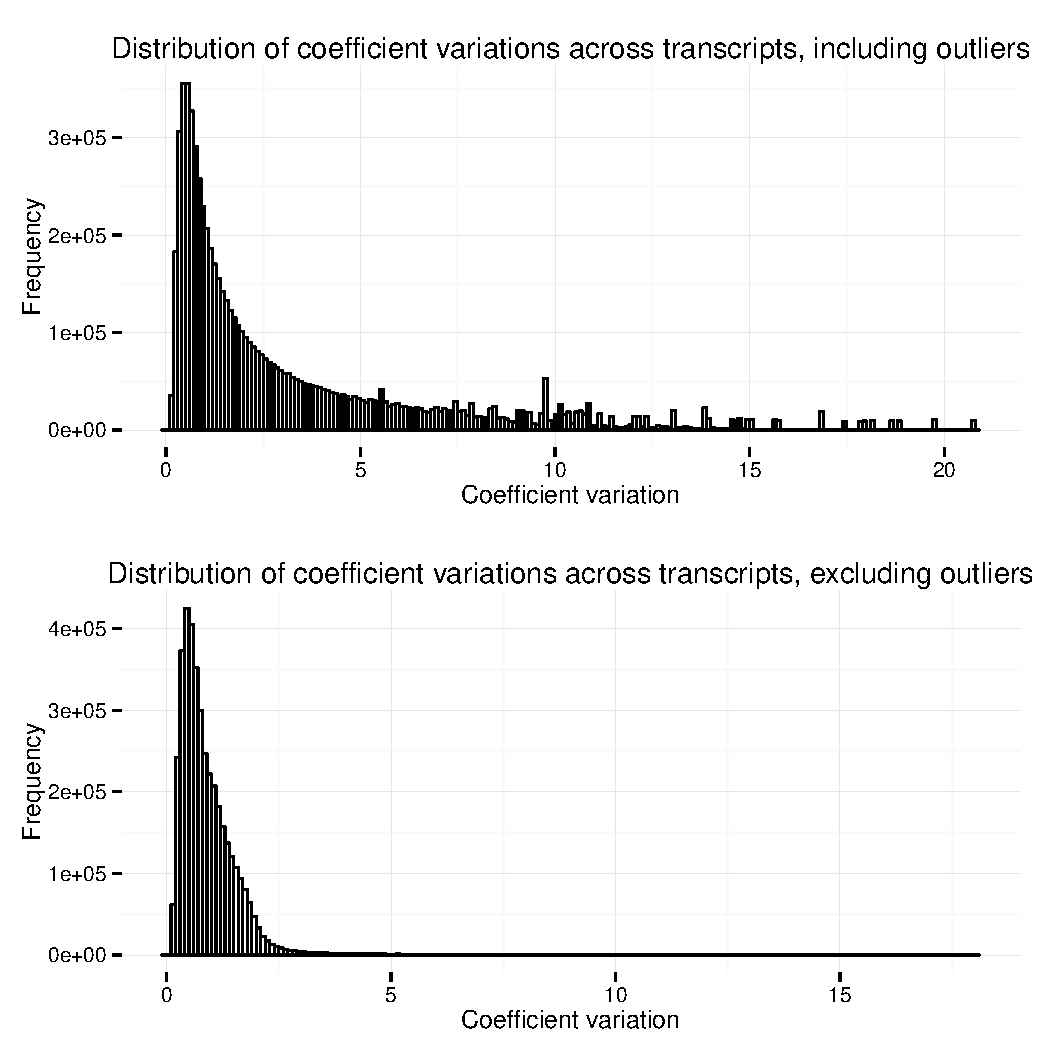
\includegraphics[width=\maxwidth]{figure/transcript_expression_averages-1} 
\begin{kframe}\begin{verbatim}
## [1] "#### Summary without removing outliers ####"
## [1] "summary(expression_df1$rpkm_mean)"
##     Min.  1st Qu.   Median     Mean  3rd Qu.     Max. 
##      0.0      0.0      0.0      4.8      0.6 702300.0 
## [1] "#### Summary removing outliers ####"
## [1] "summary(expression_df2$rpkm_mean)"
##     Min.  1st Qu.   Median     Mean  3rd Qu.     Max. 
##      0.0      0.0      0.0      4.4      0.5 406800.0 
## [1] "Plots with xlim: 5"
\end{verbatim}
\end{kframe}
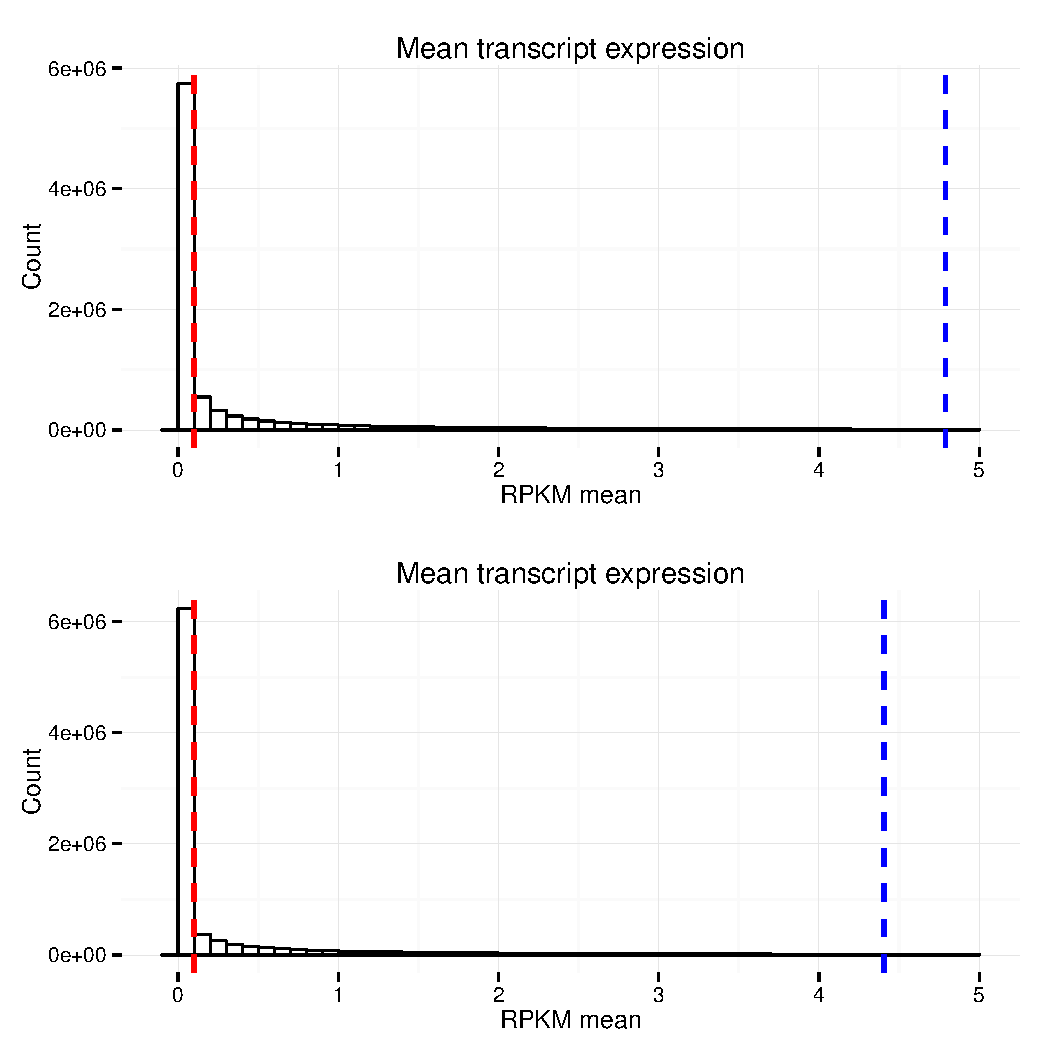
\includegraphics[width=\maxwidth]{figure/transcript_expression_averages-2} 

\end{knitrout}

From the RPKM value distributions we see that applying cutoff of 0.1 RPKM (as used in the GTEx papers) will render most transcripts in tissue as non-expressed. Also evident is the spread of the RPKM values is very high, as the mean and median are well above the values of the vast majority of transcripts. However, this is expected biologically.\par

\section{Conclusion}

We intend to use this expression data not for a (co-)expression analysis, but only as a filter layer to ensure lncRNA-protein co-existence in a cell. After setting a rpkm cutoff that distinguishes expression noise from real expression, we will turn our values into binary presence/absence.\par

TO COMPLETE

\end{document}

